\section{A codebook explains why reversal is composite}
\label{sec:domain-codebook}
\label{sec:scifact3-codebook}
On the \emph{same} 144 ContractNLI cases, we completed a $2\times2$ follow-up crossing semantic display order with label-to-answer-code assignment for Llama 3.1 8B and Qwen3 8B. The original and joint-reversal outputs were reused by exact request hash; the two missing single-factor cells were added with fixed model weights and adapter. Their messages and code maps were frozen before inference. A corrective amendment aligned the new batch size to the historical four after a batch-eight pilot had been inspected, and both pilots are retained. This is therefore a transparent follow-up diagnostic, not a wholly prospective factorial test.

The native accuracy grid (base, display-only, code-only, both) is $44,48,50,59$ correct of 144 for Llama and $65,78,63,83$ for Qwen; all 1,152 cell decisions are valid. But the semantic prediction transitions are almost orthogonal across these two model--adapter pairs. Code-only remapping changes 125/144 Llama labels (86.8\%; 95\% contract-cluster interval $[81.1,92.1]$) and only 10/144 Qwen labels (6.9\%; $[2.8,11.6]$). Display-only reversal changes 6/144 Llama labels (4.2\%; $[1.4,7.6]$) and 36/144 Qwen labels (25.0\%; $[18.1,32.2]$). Llama keeps selecting token A in 138/144 base and 131/144 code-only cases despite remapping, whereas Qwen mostly preserves semantic answers while its preferred code token changes. This is adapter-specific coupling, not a model-family mechanism.

The historical joint reversal also changes the decoder's priority for exactly tied BF16 logits. Figure~\ref{fig:codebook-main} uses one \emph{common semantic tie-break} for a comparable four-cell view, explicitly post hoc. Native counts above remain the primary reproducible record. Under this sensitivity the joint accuracy effects are $+9.0$ points for Llama and $+13.2$ for Qwen; the difference-in-differences intervals include zero in both models, so we do not claim an identified interaction. Exact repeats produce no flips. The batch-eight pilot changes three Qwen display-only predictions, underscoring the need to pin execution shape. Full tie counts and pilot details appear in Appendix~\ref{sec:codebook}.

\begin{figure}[H]
\centering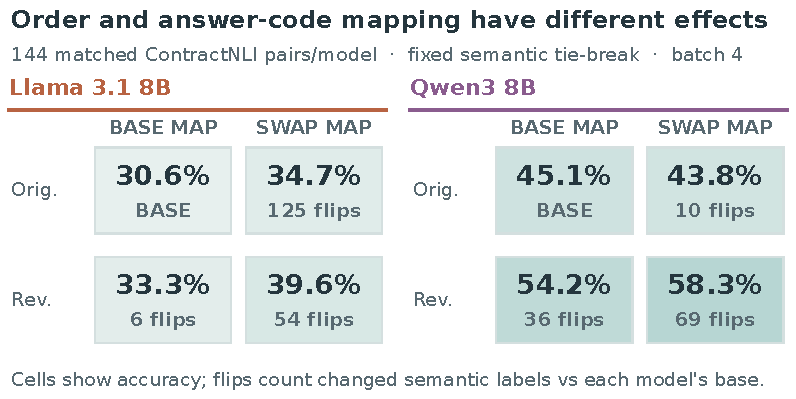
\includegraphics[width=.93\linewidth]{figures/fig_domain_codebook_main.pdf}
\caption{Orthogonal ContractNLI display-order $\times$ label-to-code control on the same 144 cases per pinned 8B adapter (historical batch size four). Cells show accuracy; switches are semantic changes from base. The grid uses a fixed semantic tie-break as an explicit post-hoc sensitivity; native joint-reversal accuracies remain 59/144 for Llama and 83/144 for Qwen. This adapter-level probe does not establish a model-family mechanism.}
\label{fig:codebook-main}
\end{figure}

A further, explicitly exploratory four-cell follow-up on the same 180 three-class SciFact cited pairs shows why the factors cannot be inferred from the joint result; we focus here on Qwen, with the second adapter reported in the supplement. The two new single-factor cells were frozen before inference; historical base/joint tokenized prompts were hash-matched, all four cells used batch size four, and Qwen's native and common-tie decisions agree. Its base, display-only, code-only and both conditions have $104,114,114,101$ reference-correct decisions. Each isolated change gains 10/180 correct cases ($+5.6$ points), whereas their joint change loses 3/180 ($-1.7$ points). Semantic label flips from base are 30, 18 and 60, respectively; the paired accuracy difference-in-differences is $-12.8$ points (claim-cluster 95\% interval $[-19.4,-6.1]$). This is non-additivity in one pinned model--adapter--task combination, not an architectural mechanism or a universal codebook effect. The follow-up was designed after the three-class result had been inspected, so its interval is descriptive rather than confirmatory.
